\section{Lemmatization and part-of-speech tagging}
\label{chap:tag}
Lemmatization and \acrlong{pos} tagging tasks are categorized as morphological analysis, shares same architecture and trained network and they will be described together in this section.
\subsection{Task Definition}

\paragraph{\textbf{POS tagging}} \mbox{}\\
\textit{input}: a sequence of  words \\
\textit{output}: tag (for each word), which contains not only part-of-speech (e.g. noun, pronoun, punctuation mark) but also other morphological analysis (case, tense, etc) corresponding to 15-places morphological tagging system by \cite{Hajic2004}. Description of each position can be found in Table \ref{Tab:tagset}.

\paragraph{\textbf{Lemmatization}} \mbox{}\\
\textit{input:} a sequence of words \\
\textit{output:} lemma -- a base form of a given words, for example nominative of singular for nouns or infinitive for verbs. In this work, lemmatization is treated as a classification problem with classes coresponding to generating rules which transform an input word into target lemma. For example of such rules see Figure \ref{fig:lemma_rules}. \\

\begin{table}[!ht]
\centering
\begin{tabular}{ |c|c|c| } 
 \hline
 Position & Name & Description \\ 
 \hline \hline
 1 & POS & Part of speech \\ \hline
 2 & SubPOS & Detailed part of speech \\ \hline
  3 & Gender & Gender \\ \hline
4 & Number & Number \\\hline
  5 & Case & Case \\ \hline
 6 & PossGender & Possessor's gender \\\hline
  7 & PossNumber & Possessor's number \\ \hline
8 & Person & Person \\\hline
  9 & Tense & Tense \\ \hline
 10 & Grade & Degree of comparison\\\hline
  11 & Negation & Negation \\ \hline
 12 & Voice & Voice \\\hline
 13 & Reserve1 & Reserve \\ \hline
14 & Reserve2 & Reserve \\\hline
  15 & Var & Variant, style \\ 
 \hline
\end{tabular}
\caption{Czech morphology developement is dated from 1989 \citep{Hajic2004} 
and in description of words uses 15-places morphological tags as described in this table taken from \url{https://ufal.mff.cuni.cz/pdt2.0/doc/manuals/en/m-layer/html/ch02s02s01.html}. For more detailed  description or for exploration of predictions given by this work is recommended to use website of Institute of Theoretical and Computational linguistics: \url{http://utkl.ff.cuni.cz/~skoumal/morfo/?pos=11\&val=1}}
\label{Tab:tagset}
\end{table}

\paragraph{Metrics} Accuracy is used for the evaluation and is reported separately for several options -- only tags/lemmas, accuracy of joint classification of tags and lemmas, and  also all three variants with an usage of a morphological dictionary (this option is described in more detail in \ref{sub:dataset}).

\begin{figure}[!ht]
\centering
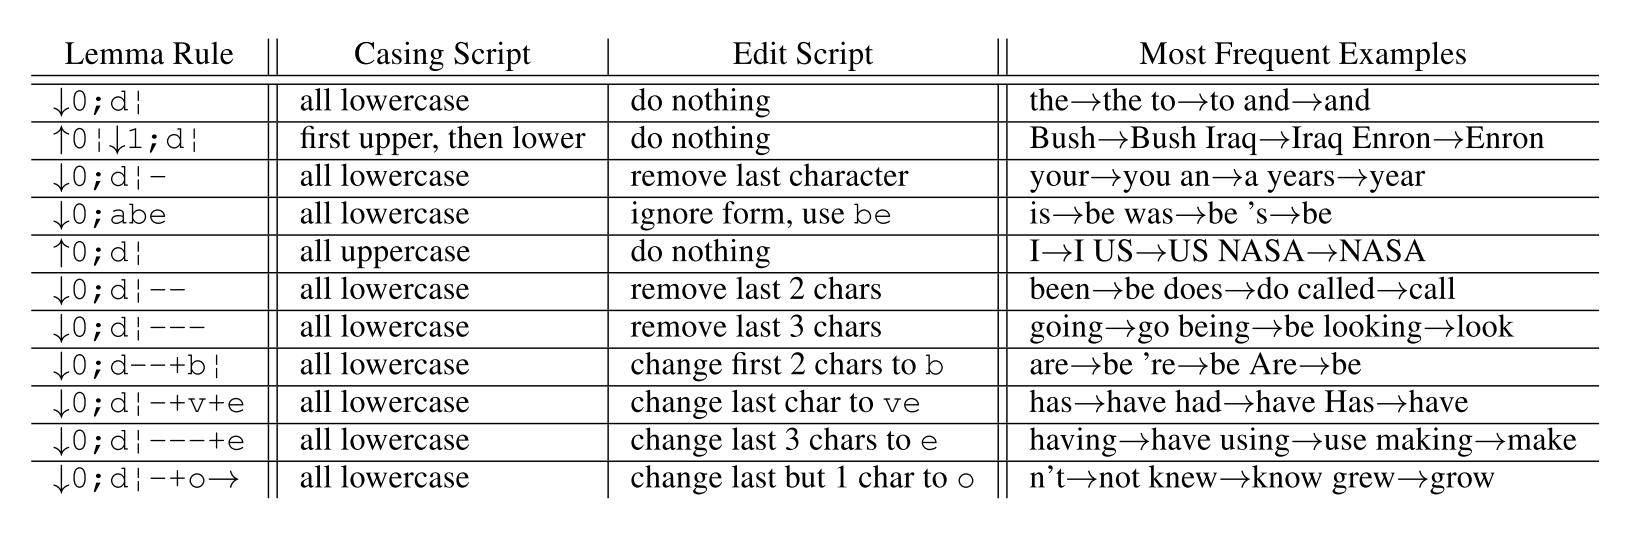
\includegraphics[width=1\textwidth]{../img/lemma_rules}
\protect\caption{
Table 1 from \citep{Straka2019b} presents 10 most common lemma generating rules in English EWT corpus. Each rule has two parts -- casing script for transforming uppercase and lowercase letters, and edit script. Edit script can transform prefix, suffix, or also a root of the word. It uses the Wagner–Fischer algorithm \citep{Wagner}, which finds the longest commont substring between the word and its lemma. Resulting rule is the shortest edit script converting the word into the lemma. More information can be found in \citep{Straka2019b}.
}
\label{fig:lemma_rules}
\end{figure}

\subsection{Related Work}
\subsubsection{Tagging}
This work aims to improve previously published SOTA results for contextualized embeddings in Czech lemmatization and tagging \citep{straka2019czech} and \citep{Straka2021}. POS tagging (for English) is dated back to 1971 with first rule-based approach on Brown Corpus \citep{greene1971automatic}. Good results in POS tagging were achieved after year 2000 using both classical machine learning methods like Hidden Markov Models \citep{tnt} or Support Vector Machines \citep{svmtool}, and perceptrons/neural networks \citep{collins-2002-discriminative}. Actual English \acrlong{sota} known to me is presented in Flair model \citep{Akbik2018}\footnote{More detailed overvirew of English tagging can be found here: https://aclweb.org/aclwiki/}. It is necessary to note that first papers had \acrshort{pos} tagging defined differently than it is in this work. They focused only on selecting part fo speech (noun, verb etc...), meanwhile later works (including this thesis) presents complex morphological analysis.
\par
One of first automatic tagging experiments in Czech is described in \citep{Hladka}, which also shows differences between languages with rich inflexion (as Czech,  but also Finnish or Turkish) and ones with more simple morphology (for example English or Spanish). Languages with complicated morphology has incomparably larger set of possible tags -- English has less then one hundred of possible tags, Czech has almost $4,000$ tags.  Current \acrshort{sota} results for tagging (and lemmatization) are presented in \citep{Straka2021}, which uses Czech version of RoBERTa model -- RobeCzech. This is the model also used for some experiments in this work and, as expected,  yields best results. RobeCzech is based upon previous successful morphological analysis with contextual embeddings and BERT-like models \citep{Straka2019b}, \citep{Straka2019a}, \citep{Straka2019}, \citep{Straka2018} (all lastly mentioned models also achieved great results in lemmatization). \par
Although tagging is mostly considered to be a classification into predifined set of tags, the sets themselves can vary. Penn treebank uses a tagset of 54 different tags, which presents parts of speech and additional informations like tense or number \footnote{see: \url{https://www.sketchengine.eu/penn-treebank-tagset/}}. There are some differences between this tagset and other English datasets or taggers (e.g. TreeTagger \citep{Schmid95improvementsin} or CLAWS tagset \citep{Chapelle1988TheCA}). All English tagsets are really small comparing to languages like Czech or Turkish. As mentioned before, Czech uses 15-positioning tags, which is  natural solution for such type of language. These positions can be predicted together or for each position separately. First approach creates big tagset but guarantees consistency among positions (e.g. there will be no tense for a noun or a case for a verb). In the case of separate prediction, each position can be treated as a classification problem separately, which causes problems, because the individual parts of tag are not independent. Better approach is to use sequence-to-sequence modelling \citep{Sutskever2014}, which outputs the tag as a sequence of positions and takes into account previously generated position as in \citep{malaviya-etal-2019-simple}.

\subsubsection{Lemmatization}
Lemmatization (both Czech and English) has undergone a similar development as tagging, starting with rule-based approaches and statistical approaches \citep{Plisson}, continuing with neural networks and recently achieving good results with BERT-like models \citep{Kondratyuk2019}.  Lemmatization is typically performed as a sequence-to-sequence model, therefore it takes a word as a sequence of characters and produces a new sequence of characters, which is the lemma. This approach is teoretically better than classification into rules, because it is possible to generate every existing lemma. However, it can generate simply every possible character sequence, which may not be an existing word. Lemmatization as a classification task into edit scripts set firstly appeared in \citep{Chrupala} and more explored by \citep{Straka2018}. 
Sequence-to-sequence model can be also used for production of edit rules (same rules as used in this work)\citep{chakrabarty2017context}, \citep{muller2015joint} and \citep{Yildiz2019}.

\subsection{Dataset and Preprocessing}
\label{sub:dataset}
Dataset for these tasks is taken from data of Prague Dependency Treebank (PDT) \citep{PDT35}, version 3.5 from year 2018. Data consists of sentences with lemmas and tags. For ambiguous words, data contain all possible analysis. For example, Czech word "psa" have one possible lemma ("pes") but two possible tags because it could be one of two possible grammatical cases -- genitive or accusative. Input data for such word looks as follows: \\
\begin{center}
\texttt{psa pes NNMS2-----A---- NNMS4-----A----}.
\end{center}
Data contains about 1,600 unique tags and 15k different lemma rules. The number of lemmas is significantly smaller than a number of unigue lemmas ($72,000$) \citep{Strakova} or tags, because words with similar morphological function have same way of creating lemma from the word, e.g. words \textit{malého} (=little, accusative,  sg, m.,) and \textit{červeného}  (=red, accusative,  sg, m.,) have the same lemma rule:
\begin{center}
\texttt{$\downarrow$ 0;d\textbrokenbar ---+ý+-+1}.
\end{center} 
\par
Dataset was originally divided into tree parts - train, development and test, which is also used in this work. Input sentences are preprocessed as follows:
\begin{itemize}
\item white space deletion
\item splitting into sentences and words
\item mapping characters and words into numbers -- mapping  words/characters which were found in train dataset into integers (from one to the number of unique words). This means that the network has no information about words/characters which appears only in test or development dataset. All newly appeared words/characters are mapped into one same number (typically $0$) for \textit{UNK} token/character.
\item tokenization -- Tokenizer for corresponding BERT-like model transforms input words into tokens. Each word is transformed into one or more strings, which are converted into numbers. This serves as an input into BERT part of model. To creating these input embeddings, the whole sentence for each word is needed as same words can have different representation in different contexts. More information can be found in \ref{sub:tokens}.
\end{itemize}

\subsection{Architecture and Experiments}

\begin{figure}[!h]
\centering
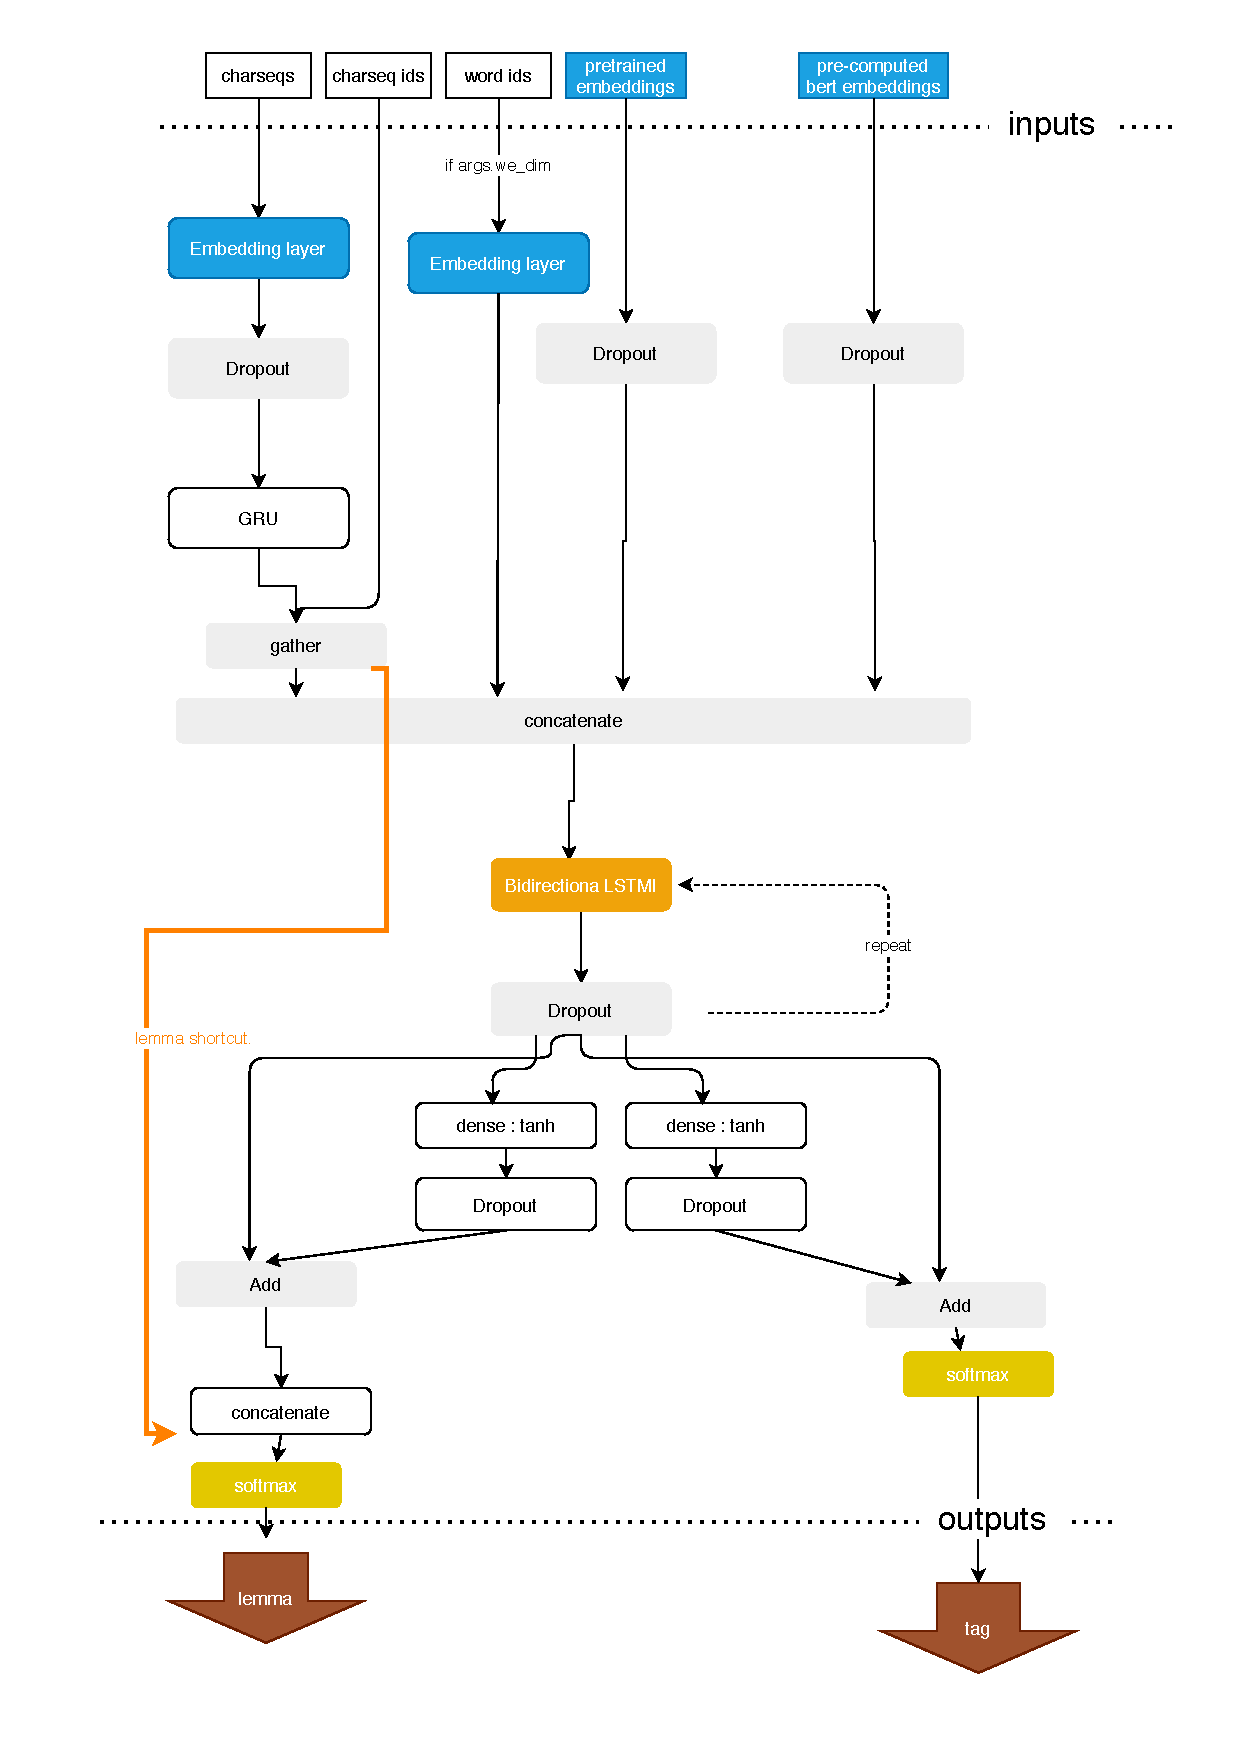
\includegraphics[width=1\columnwidth]{../img/taggermodel.pdf}
\protect\caption{Tagging and lemmatization joint model architecture.}
\label{pic:lt_arch}
\end{figure}
%TODO kolik je tech lstm a tak,vsechny dimenze (do tabulky)

%For POS tagging, we applied a straightforward model in the lines of Ling et al. (2015) – first rep- resenting each word with its embedding, contextu- alizing them with bidirectional RNNs (Graves and Schmidhuber, 2005), and finally using a softmax classifier to predict the tags. z UDpipe2

The model for lemmatization and tagging is build upon a model (and a code) for previous work on Czech NLP processing with contextual embedding \citep{straka2019czech}. 
Data preprocessing is taken over from the paper as well as the structure of a lemmatizer and a tagger network, which is extended by BERT-like models, hoping for improvements. %TODO k tomu nemam citaci
Previous work showed that training tagging and lemmatization together in one network can be mutually advantageous, so both of these analysis are an output of one network and are trained jointly. Detailed visualisation of network architecture can be found in Figure \ref{pic:lt_arch}. \par The architecture of network can be divided into three parts -- inputs, optional \acrshort{rnn}s, classification head:
\paragraph{Inputs}
An input of the network is formed of five types -- characters (charseqs), words (charseq ids), correct responses(word ids), pretrained embeddings and possibly precomputed bert embeddings (depends on the experiment type). Before the further processing of inputs by \acrshort{rnn} cells, there are created two other types of embeddings: character-level embeddings and another word embeddings which are, in contrast to BERT and pretrained embeddings, also trained during training process.

\paragraph{RNN cells}
Characterlevel embeddings are further processed via 3 layers of \acrfull{gru} and all inputs (or their embeddings) are processed by recurrent part of network (specifically by \acrfull{lstm} cells).

\paragraph{Classification head(s)}
After the processing by recurrent neural networks, network employs two separate classification head, one for tagging and another for lemmatization. Both uses dense layer with tanh activation function to presented more non-linearity as used in \citep{Straka2018} and a softmax function for obtaining the probability distribution over target classes. Lemmatization, however, presents one another change -- addition of character level data without RNN processing, which are used together with the rest of weights as an input into softmax following \citep{Straka2018}, because it leads to better performance of lemmatization in the case of shared network between both tasks.

%TODO kondraytuk bere predikci k prvnímu subwordu, jak to delam ja? 


\paragraph{Morphological Dictionary} All classification can be done with or without use of a morphological dictionary MorFlex \citep{11234/1-1834}, which can provide possible pairs \textit{tag-lemma}. If so, generated tag and lemma is a pair with maximal likelihood, but chosen just from the dictionary. This leads to more consistent results. 


%TODO nekde mam taky dropouts! zminit
\subsubsection{Experiments}
This part uses all main \textbf{experiment types} as decribed in \ref{sec:expe}: \textit{base, ls, embed, fine, simple} and \textit{full}. Three \textbf{BERT-like models} are used for experiment setup:
\begin{itemize}
\item multilingual BERT (mBERT) \citep{Devlin2019} 
\item XLM-RoBERTa \citep{Conneau2019}), 
\item RobeCzech \citep{Straka2021}.
\end{itemize}
XLM-RoBERTa and mBERT are trained on 100/104 different languages including Czech. RobeCzech is recently published version of RoBERTa,, trained only on Czech data. XLM-RobERTa is used only for embedding and one version of finetunnig and this model was omitted in other experiements because of weak results and high computational complexity. There exists another monolingual Czech model, Czert \citep{Sido2021}, which uses original BERT architecture and was outperformed by Robeczech \citep{Straka2021}. \par
A selection of layers is made in both ways -- last four layers (\textit{four)} and learning of weighted sum of all layers (\textit{att}). The layer attention is made only for finetunning setup and as the weighted sum does not showed a significant benefit, mean of last four layer is the only method used for other experiments.
 \par Learning rate is used as usual for each type of task a and three different learning rate schedules were applied in each combination of hyperparameters: cosine decay \textit{(cos)}, inverted square root decay \textit{(isrd)} and a one epoch warm-up followed by a constant learning rate \textit{(warmup)} inspired by \citep{Kondratyuk2019} and \citep{Ruder2018}. For \textit{embed} experiments, \textit{warmup} is replaced by  a simple division of training into two parts with different learning rates. 
 
 \begin{table}[!h]
 \centering
\begin{tabular}{|l||l|}
\hline
hyperparametr   & \multicolumn{1}{l|}{value} \\ \hline \hline
beta\_2          & 0.99                       \\ \hline
optimizer       & Adam                       \\ \hline
cle\_dim         & 256                        \\ \hline
dropout         & 0.5                        \\ \hline
label smoothing & 0.3                        \\ \hline
rnn\_cell        & LSTM                       \\ \hline
rnn\_cell\_dim    & 512                        \\ \hline
rnn\_layers      & 3                          \\ \hline
we\_dim          & 512                        \\ \hline
word\_dropout    & 0.2                        \\ \hline
batch size & 64 \\ \hline
\end{tabular}
\caption{Hyperparameters of tag and lemmatization common to all experiments (if they make sense in the context of experiments).}
\label{tab:hyp_all}
\end{table}
Batches has size 64, given by the compromise between the pursuit of relatively big batch size and computational resources. Summary of hyperparameters, which not different across experiments are in the table \ref{tab:hyp_all}. Other hyperparameters for each experiment are in Appendix \ref{att:1}.
\par 
Reimplementation of \citep{Straka2019c} without any BERT-like model incorporation serves as a baseline.

\subsection{Results and Discussion}
Best presented model (experiment no. 18) achieved same or better results than current \acrlong{sota} tagging and lemmatization results (table \ref{tab:all_prew}). Complete result are in table \ref{tab:all_res_tl}. \textit{best(18} is the version with finetunning, Czech monolingual model, RobeCzech and without layer attention, although the difference from comparable experiment \textit{with} layer attention is insignificant and can be just accidental. The dominance of the Czech model was expected and additional expert knowledge contained in the complicated architecture was also assumed to be better. Experiments also showed that finetunning approach achieves better results than full training from the beginning. This may be due to the choice of hyperparameters, especially learning rate, but  we chose the standard ones, therefore finding right parameters is at least more difficult in the case of \textit{full} and \textit{simple} variants.  %TODO a jak je to s finetuning vs full vs simple? %TODO co jeste?

\begin{table}[!h]
\centering
  \begin{tabular}{|l||ccc||ccc|}
  \hline
\multirow{2}{*}{Experiment} & \multicolumn{3}{c||}{Without Dictionary}  &
      \multicolumn{3}{c|}{With Dictionary} \\ 
    & Tags & Lemmas & Both & Tags & Lemmas & Both \\ \hline \hline
    \textit{StrakaB} & \textit{97.94} & \textit{98.75} & \textit{97.31} & \textit{98.05} & \textit{98.98} & \textit{97.65 }\\ \hline
   \textit{ StrakaC} & \textit{97.67} & \textit{98.63} & \textit{97.02} & \textit{97.91 }& \textit{98.94} & \textit{97.51} \\ \hline
     \textit{RobeCzech} & \textit{98.43} & \textit{98.79}  & \textit{97.83}  & \textit{98.50} & \textbf{99.00}  & \textit{98.11} \\ \hline \hline
      baseline & 97.04  & 98.56  & 96.41 &  97.31   & 98.83  & 96.90 \\ \hline 
    emb(12) & 98.38  &98.79  & 97.80 & 98.48  & 98.99 & 98.10 \\ \hline
    best(18) & \textbf{98.50}  & \textbf{98.80} &\textbf{ 97.90}  & \textbf{98.57}  & \textbf{99.00}  & \textbf{98.19}  \\ \hline  
  \end{tabular}
  \caption{%TODO cite
  \textit{Straka2019B} is the best solution from \citep{Straka2019} paper. \textit{Straka2019C} is a comparable solution  (BERT embeddings only) to \textit{emb}, which was transformed into Tensorflow 2 in this work as a \textit{baseline}. \textit{Emb} is a solution with static BERT embeddings and \textit{best(18) is the best resulting model in this thesis (18 is an id of experiment.). }}
\label{tab:all_prew} 
\end{table}

\begin{table}[!h]
\resizebox{\columnwidth}{!}{% Please add the following required packages to your document preamble:
% \usepackage{multirow}
\begin{tabular}{|l|l|l|l||llllll|}
\hline
\multicolumn{2}{|c|}{Model}                      & EXPE                    & LRTYPE & LemR & LemD & TagsR & TagsD & JointR & JointD \\ \hline \hline
0  & NA                           & base                    & simple & 98.58  & 98.81   & 97.05   & 97.31    & 96.43     & 96.9       \\ \hline
1  & NA                           & ls                      & simple & 98.55  & 98.81   & 97.12   & 97.34    & 96.51     & 96.94      \\ \hline
2  & \multirow{3}{*}{mBERT}       & \multirow{9}{*}{embed}  & simple & 98.69  & 98.93   & 97.83   & 97.98    & 97.17     & 97.58      \\ \cline{1-1} \cline{4-10}
3  &                              &                         & cos    & 98.74  & 98.95   & 97.91   & 98.04    & 97.28     & 97.63      \\ \cline{1-1} \cline{4-10}
4  &                              &                         & isrd   & 98.73  & 98.94   & 97.89   & 98.02    & 97.28     & 97.61      \\ \cline{1-2} \cline{4-10}
5  & \multirow{3}{*}{xlm-Roberta} &                         & simple & 98.57  & 98.8    & 97.33   & 97.54    & 96.68     & 97.12      \\ \cline{1-1} \cline{4-10}
6  &                              &                         & cos    & 98.6   & 98.83   & 97.45   & 97.62    & 96.81     & 97.21      \\ \cline{1-1} \cline{4-10}
7  &                              &                         & isrd   & 98.59  & 98.83   & 97.44   & 97.61    & 96.81     & 97.2       \\ \cline{1-2} \cline{4-10}
8  & \multirow{3}{*}{RoBECzech}   &                         & simple & 98.77  & 98.97   & 98.38   & 98.48    & 97.78     & 98.08      \\ \cline{1-1} \cline{4-10}
9  &                              &                         & cos    & 98.79  & 98.99   & 98.38   & 98.48    & 97.8      & 98.1       \\ \cline{1-1} \cline{4-10}
10 &                              &                         & isrd   & 98.78  & 98.98   & 98.4    & 98.48    & 97.8      & 98.09      \\ \hline
11 & \multirow{3}{*}{mBERT} & \multirow{9}{*}{fine} & simple & 98.69 & 98.93 & 97.84 & 97.99 & 97.21 & 97.59 \\ \cline{1-1} \cline{4-10}
12 &                              &                         & cos    & 98.72  & 98.95   & 97.97   & 98.08    & 97.33     & 97.68      \\ \cline{1-1} \cline{4-10}
13 &                              &                         & isrd   & 98.68  & 98.9    & 97.72   & 97.86    & 97.09     & 97.46      \\ \cline{1-2} \cline{4-10}
14 & \multirow{3}{*}{xlm-Roberta} &                         & simple & 98.62  & 98.84   & 97.72   & 97.9     & 97.07     & 97.48      \\ \cline{1-1} \cline{4-10}
15 &                              &                         & cos    & 98.67  & 98.9    & 97.95   & 98.09    & 97.32     & 97.69      \\ \cline{1-1} \cline{4-10}
16 &                              &                         & isrd   & 98.63  & 98.85   & 97.66   & 97.83    & 97.03     & 97.41      \\ \cline{1-2} \cline{4-10}
17 & \multirow{3}{*}{RoBECzech}   &                         & simple & 98.78  & 98.98   & 98.46   & 98.55    & 97.86     & 98.16      \\ \cline{1-1} \cline{4-10}
18 &                              &                         & cos    & \textbf{98.8}   & \textbf{99 }     & \textbf{98.5}    & \textbf{98.57}    & \textbf{97.9 }     & \textbf{98.19 }     \\ \cline{1-1} \cline{4-10}
19 &                              &                         & isrd   & 98.76  & 98.95   & 98.33   & 98.41    & 97.72     & 98.02      \\ \cline{1-2} \cline{4-10} \hline
20 & \multirow{3}{*}{mBERT}       &      \multirow{9}{*}{fine att}                    & simple & 98.67  & 98.91   & 97.76   & 97.92    & 97.13     & 97.52      \\ \cline{1-1} \cline{4-10}
21 &                              &                         & cos    & 98.72  & 98.95   & 97.98   & 98.1     & 97.34     & 97.69      \\ \cline{1-1} \cline{4-10}
22 &                              &                         & isrd   & 98.67  & 98.91   & 97.69   & 97.85    & 97.05     & 97.45      \\ \cline{1-2} \cline{4-10}
23 & \multirow{3}{*}{xlm-Roberta} &                         & simple & 98.6   & 98.81   & 97.62   & 97.77    & 96.96     & 97.35      \\ \cline{1-1} \cline{4-10}
24 &                              &                         & cos    & 98.67  & 98.89   & 97.91   & 98.06    & 97.29     & 97.66      \\ \cline{1-1} \cline{4-10}
25 &                              &                         & isrd   & 98.65  & 98.86   & 97.65   & 97.81    & 97.03     & 97.41      \\ \cline{1-2} \cline{4-10}
26 & \multirow{3}{*}{RoBECzech}   &                         & simple & 98.77  & 98.97   & 98.38   & 98.47    & 97.79     & 98.08      \\ \cline{1-1} \cline{4-10}
27 &                              &                         & cos    & \textbf{98.8}   & 98.99   & 98.47   & 98.54    & 97.88     & 98.16      \\ \cline{1-1} \cline{4-10}
28 &                              &                         & isrd   & 98.77  & 98.96   & 98.33   & 98.41    & 97.72     & 98.01      \\ \hline
29 & \multirow{3}{*}{mBERT}       & \multirow{9}{*}{simple} & warmup & 98.17  &         & 97.32   &          & 96.46     &            \\ \cline{1-1} \cline{4-10}
30 &                              &                         & cos    & 98.15  &         & 97.39   &          & 96.47     &            \\ \cline{1-1} \cline{4-10}
31 &                              &                         & isrd   & 98.13  &         & 97.12   &          & 96.29     &            \\ \cline{1-2} \cline{4-10}
35 & \multirow{3}{*}{RoBECzech}   &                         & warmup & 98.49  &         & 98.28   &          & 97.41     &            \\ \cline{1-1} \cline{4-10}
36 &                              &                         & cos    & 98.46  &         & 98.30   &          & 97.39     &            \\ \cline{1-1} \cline{4-10}
37 &                              &                         & isrd   & 98.59  &         & 98.27   &          & 97.53     &            \\ \hline
38 & \multirow{3}{*}{mBERT}       & \multirow{9}{*}{full}   & warmup & 98.16  & 98.86   & 97.35   & 97.79    & 96.46     & 97.34      \\ \cline{1-1} \cline{4-10}
39 &                              &                         & cos    & 98.04  & 98.85   & 97.36   & 97.81    & 96.3      & 97.34      \\ \cline{1-1} \cline{4-10}
40 &                              &                         & isrd   & 98.22  & 98.86   & 97.34   & 97.73    & 96.46     & 97.29      \\ \cline{1-2} \cline{4-10}
44 & \multirow{3}{*}{RoBECzech}   &                         & warmup & 98.49  & 98.95   & 98.21   & 98.34    & 97.38     & 97.93      \\ \cline{1-1} \cline{4-10}
45 &                              &                         & cos    & 98.25  & 98.95   & 98.17   & 98.33    & 97.08     & 97.89      \\ \cline{1-1} \cline{4-10}
46 &                              &                         & isrd   & 98.55  & 98.99   & 98.19   & 98.35    & 97.39     & 97.95      \\ \hline
\end{tabular}
}
\caption{This table presents complete results for tagging and lemmatizationt tasks.  Complete hyperparameters for each experiment are in separate table in Appendix \ref{att:1}.
}
\label{tab:all_res_tl}
\end{table}

\subsubsection{Error Analysis}
This section offers a little exploration of difference between error across models. This comparison includes three models: 
\begin{itemize}
\item tl\_18 -- the best model in tagging and lemmatization,
\item tl\_3 -- the best model with mBERT,
\item tl\_1 -- the baseline model with label smoothing.
\end{itemize} 

\paragraph{best vs. baseline}
The best model (tl\_18) improved prediciton in $3,247$ tags and was worse in 421 tag predictions. More than 80\% of newly correctly predicted tags is composed by three tags of speech: NN (noun), AA (adjective) and RR (preposition). Table %TODO udelat
presents the number of improved tags divided by parts of speech and cases and table %TODO udelat
presents 10 most frequent imrpoved tags. %TODO nejaky zaver z toho? tak napriklad hned druhy a treti nejcastejsi je napriklad hrad, ktery je stejny v 1 i 4 pade, prvni jsou typicky vlasntí cizí jména (místa apod., Jersey, Tenesee), totez jako hrad pro zensky rod v pluralu


%TODO NNNXX vypsat

to je přes 80% zlepšení
NN:1760
AA:733
RR:127

na trojice tedy: 
NNF:517
NNN:512
NNI:431
NNM:290
NNX:10
AAI:235
AAF:230
AAN:139
AAM:110
AAX:19
RR-:127

a takto pády:
nn
1:577
4:557
X:230
2:189
3:86
7:57
6:57
5:7
aa
1:291
4:243
2:97
3:34
7:30
X:19
6:19
rr
4:58
6:54
2:11
X:2
7:2

tagy vetsi nez 10 vyskytu:
NNNXX-----A----:163
NNIS1-----A----:151
NNIS4-----A----:130
NNNS4-----A----:122
NNFP1-----A----:103
NNMS1-----A----:99
NNFP4-----A----:84
NNNS1-----A----:83
NNMS4-----A----:72
AAIS4----1A----:69
NNFS1-----A----:68
AAFP1----1A----:64
AAIS1----1A----:62
NNFS4-----A----:60
RR--4----------:58
NNFS2-----A----:56
RR--6----------:54
NNNS2-----A----:48
NNMS2-----A----:48
VB-P---3P-AA---:47
NNIP1-----A----:47
AANS4----1A----:47
Db-------------:43
NNIP4-----A----:42
VB-S---3P-AA---:38
NNFS3-----A----:38
AANS1----1A----:35
AAFS2----1A----:35
AAFP4----1A----:35
AAIP1----1A----:33
NNFS7-----A----:28
AAMS1----1A----:27
NNMP4-----A----:25
NNNP1-----A----:22
NNFS6-----A----:22
NNFXX-----A---8:21
NNNS6-----A----:20
PDNS1----------:19
J,-------------:19
AAIP4----1A----:19
NNNS3-----A----:18
AAFS4----1A----:18
AAFS1----1A----:17
PDNS4----------:16
NNNP4-----A----:16
NNIS3-----A----:16
AANP1----1A----:15
%J^-------------:14
NNIP7-----A----:13
NNFP2-----A----:13
Cn-S1----------:13
P7-X4----------:12
NNIS2-----A----:12
AAMP2----1A----:12
RR--2----------:11
NNMS3-----A----:11
AGFP1-----A----:11
AAXXX----1A----:11
AAMS2----1A----:11
AAFS3----1A----:11
NNFXX-----A----:10
AAMP4----1A----:10


%TODO kolik lemmata

%TODO jake chyby stejne jako predchozi porovnani
Best mbert is better in 468 tags and worse in 1703 tags than best model 
NN:862
AA:390
VB:71
RR:59
PD:48
P4:38
AG:31
Db:24
PP:23
Cn:14
Ca:13
Cr:12
RV:10
J,:10

trojice
NNF:287
NNN:222
NNI:213
NNM:130
NNX:10
AAF:139
AAI:115
AAN:75
AAM:44
AAX:17

pady:
1:148
4:125
2:61
X:17
7:14
3:13
6:12

tagy cele:
NNIS1-----A----:70
NNNS4-----A----:69
NNIS4-----A----:55
NNFP1-----A----:55
NNNS1-----A----:45
NNFS1-----A----:45
NNMS4-----A----:38
NNFP4-----A----:38
AAFP1----1A----:37
NNFS2-----A----:36
NNFS4-----A----:34
VB-S---3P-AA---:32
AAIS1----1A----:30
VB-P---3P-AA---:29
RR--4----------:28
NNNXX-----A----:27
NNMS2-----A----:27
AAIS4----1A----:27
NNNS2-----A----:26
AANS4----1A----:26
NNMS1-----A----:25
NNIP4-----A----:23
Db-------------:23
AAFS2----1A----:23
RR--6----------:22
NNIP1-----A----:22
NNFS3-----A----:21
AANS1----1A----:20
AAIP1----1A----:16
NNNS3-----A----:15
NNFXX-----A---8:15
NNFS7-----A----:15
AAFP4----1A----:15
PDNS1----------:13
NNIS3-----A----:13
AAIP4----1A----:13
PDNS4----------:12
NNNS6-----A----:11
AAFS4----1A----:11
NNMP4-----A----:10
J,-------------:10
AAXXX----1A----:10
AAMS1----1A----:10
%TODO kolik lemmata
